% !TEX root = cikm2018-visual-ltr.tex

\section{Method}
In this section we proposing a multimodal architecture used to train a \ac{LTR} model with both visual and content features. 
Secondly, we demonstrate how the architecture can be exploited to drastically reduce the computational costs during training. 
The three paragraphs that follow decribe the implementation of three visual feature extractors, being:
\begin{inparaenum}[(i)]
\item the ViP baseline model proposed in~\citet{fan2017learning}, 
\item the VGG-16~\cite{simonyan2014very} classification model pretrained on ImageNet, and
\item the ResNet-152~\cite{he2016deep} classification model pretrained on ImageNet.
\end{inparaenum} 
Finally, we propose the use of a saliency model to create synthetic saliency heatmaps for each of the input images, in order to create a more expressive representation of the interaction of a user. 

All corresponding code is available on Github.\footnote{URL removed for review}

\paragraph{Multimodal architecture}
In order to compare the performance of various visual feature extractor methods, we propose a reusable multimodal architecture. 
The multimodal architecture is visualized in Figure~\ref{fig:multimodelarchitecture}. 
The model starts by taking an image $x_{v}$ (1) as an input to the visual feature extraction layer (2) in order to create a generic visual feature vector $x_{vf}$. In turn, $x_{vf}$ is then used as an input to the visual feature transformation layer (3).
This visual feature transformation layer learns to transforms the generic visual features to a \ac{LTR} specific visual feature vector $x_{vl}$.

The final \ac{LTR} feature vector $x_{l}$ is constructed by concatenting the visual \ac{LTR} features $x_{vl}$ with the content \ac{LTR} features $x_{c}$ (4). 

$x_{l}$ is then used as an input to the scoring component (5), which transforms the features to a single score for each document-query pair. The scoring component uses a single fully connected layer with a hidden size of $10$ with dropout imperically set to $10\%$. The resulting model is trained end-to-end using a pairwise hinge loss with $L_2$ regularization. 

% \begin{multline}
% x_{vl} = f_{t}(f_{v}(x_{v})) \\ x_{s} = f_{s}(x_{vl} \oplus x_{c}) 
% \end{multline}

\paragraph{Reducing training complexity}
Both training and inference using deep convolutional networks are generally computationally expensive.
By separating the network in a visual feature extraction and transformation layer as described above, we can drastically reduce the computational requirements by freezing the parameters of the extractor layers.
To even further reduce the memory and computational cost during training, we can store the $x_{vf}$ vectors to disk prior to training, allowing us to replace $x_{v}$ with the much smaller $x_{vf}$ as an input to the model and removing the parameters of the visual feature extractor completely during training.

% VGG16 -  	  	   134,383,885
% VGG16 cached:    119,669,197
% difference    	14,714,688

% ResNet-152 	    58,205,709
% ResNet-cached   	   	61,470
% ResNet-modified 	59,243,247
% difference 	    58,144,239

% scores network with images: 750
% scorer network no images: 450

\begin{figure}[t]
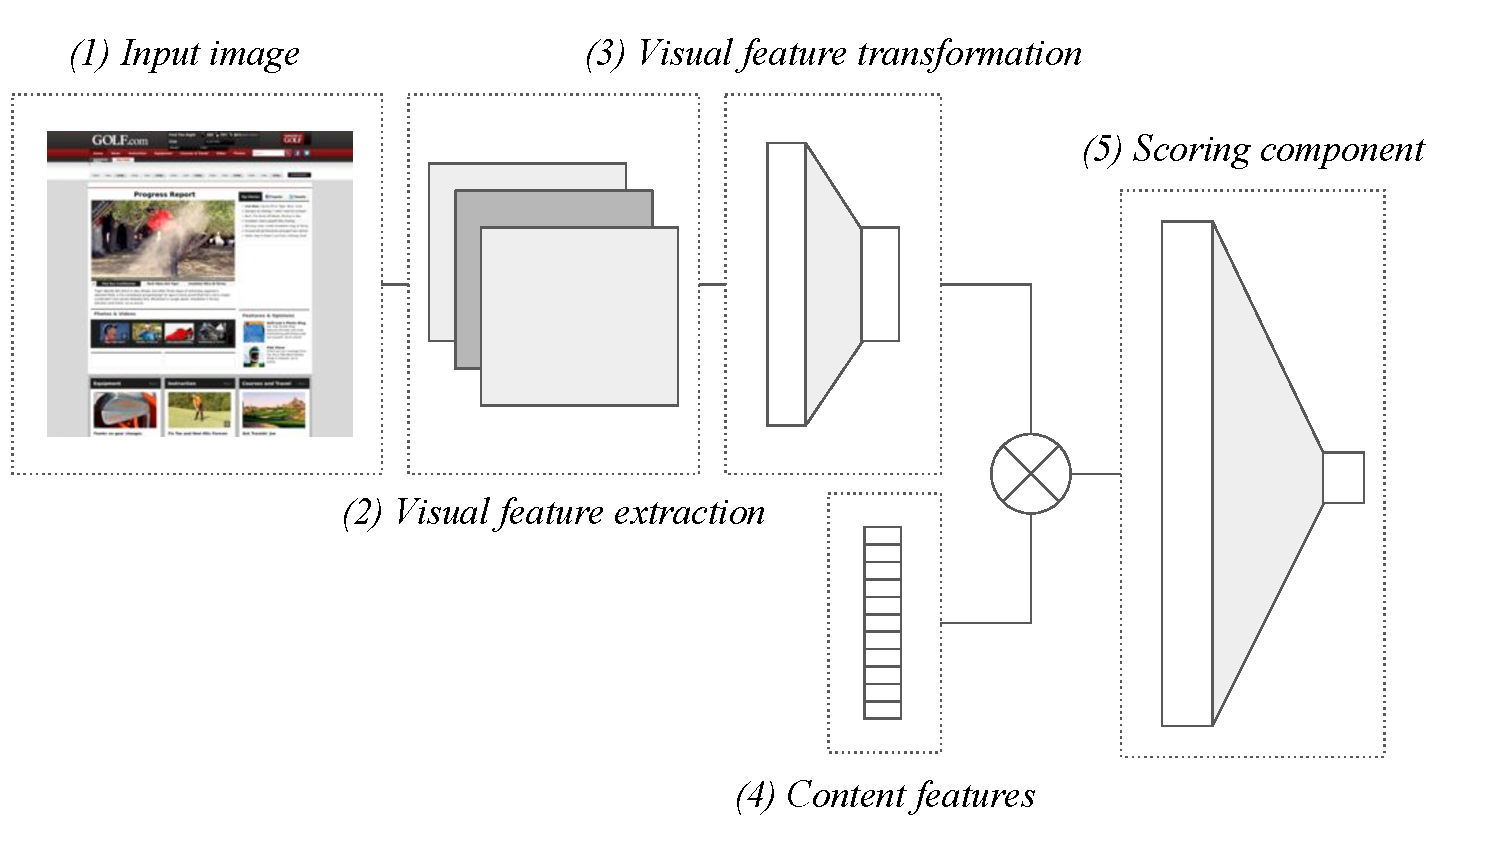
\includegraphics[width = 3.5in]{images/multimodelarchitecture.pdf}
\caption{The proposed multimodal architecture, which the visual feature extraction}
\label{fig:multimodelarchitecture}
\end{figure}

\paragraph{ViP visual features}
As a baseline, we implement the visual feature extractor proposed in~\citet{fan2017learning} using PyTorch.
In this model, $x_{v}$ is gray-scaled, normalized and horizontally segmented into $4\times16$ slices before being processed by the visual feature extractor. The visual feature extractor processes all slices separately using a shallow convolutional network.
Each of these outputs is then being passed from top to bottom through an LSTM in order to create $x_{l}$.

\paragraph{VGG-16 visual features}
Since the \datasetname{} data\-set that we introduce in this paper has a relatively low number of snapshots to train a separate feature extractor, we use the VGG-16 model~\cite{simonyan2014very} from Torchvision,\footnote{\url{https://github.com/pytorch/vision/blob/master/torchvision/models/vgg.py}} pretrained on ImageNet, as a feature extractor. 
Although VGG-16 is not the current state-of-the-art visual feature extractor, it is a reasonable trade-off between effectiveness and simplicity.
The VGG-16 architecture consists of a set of convolutional filters and fully connected layers. 
The convolutional filters extract features from the input image, which are used by the fully connected layers to classify the image. 
These filters are generic with respect to input and task~\citep{donahue2014decaf}, which make them suitable for being used as a visual feature extractor to create generic visual features $x_{vf}$. The fully connected layers can be altered and retrained in order to be used with new inputs and tasks, making them suitable to be used as a visual feature transformation layer.

As described above, we transform all input images using the convolutional layers prior to training, changing all $3\times224\times224$ input images to a single vector of $1\times25088$ reducing the input size by $84.7\%$ and removing all convolutional parameters. The remaining fully connected layers are retrained, with the last fully connected layer reinitialized to produce $x_{img\_ltr}$. The size of $x_{img\_ltr}$ was set to $30$ which was empirically found to provide good performance in preliminary results.

% TODO: Bring this back? VGG-16 uses a $224\times224$ image with three color channels as input as opposed to the gray-scaled $64\times64$ input used by ViP, giving us the advantage that both color and low-level features persist. 

\paragraph{ResNet-152 visual features}
The ResNet-152~\cite{he2016deep} architecture has a significant increase in image classification performance over VGG-16. The residual connections between convolutional layers allow for deeper networks to be trained without suffering from vanishing gradients. Similar as with the VGG-16 model, we use the convolutional layers to convert each $3\times224\times224$ input image to $x_{vf}$ prior to training, which has a size of only $1\times2048$ reducing the input size by $98.6\%$. The original ResNet-152 architecture only has a single fully connected layer, which empirically showed not be enough to successfully train the model. Instead, we train a fully connected network from scratch. The network was constructed using three layers with $4096$ hidden units and a final layer resulting in $x_{img\_ltr}$ with a size of $30$, which was empirically found to provide good performance in preliminary results.


\paragraph{Saliency heatmaps}
In order to increase the ability to learn the visual quality of a webpage, we propose to explicitly model the user viewing pattern by using synthetic saliency heatmaps. 
Following \cite{shan2017two}, we implemented and trained a two-stage transfer learning model that learns how to predict saliency heatmaps on webpages.
Similarly to the visual feature extraction approaches in the paragraphs above, \cite{shan2017two} takes a pretrained image recognition model and finetunes the output layers on the following two datasets in order respectively:
\begin{inparaenum}[(i)]
\item SALICON by \cite{jiang2015salicon}, a large dataset containing saliency heatmaps created with eye-tracking hardware on natural images, and 
\item the webpage saliency dataset by \cite{shen2014webpage}, a smaller dataset containing saliency heatmaps created with eye-tracking hardware on webpages.
\end{inparaenum}

The trained model is applied to the $3\times224\times224$ input images from the \datasetname data\-set, resulting in grayscale heatmaps with a dimension of $1\times64\times64$. These heatmaps can then be used as the $x_{v}$ for the visual feature extractors described above by linearly scaling them to $3\times224\times224$, matching them with the VGG-16 and ResNet-152 input dimensions. Figure~\ref{fig:exampleshots} shows example snapshots with their corresponding saliency heatmaps.

The saliency heatmaps generated using this method have various advantages over the usage of vanilla and keyword highlighted snapshots because synthetic saliency heatmaps
\begin{inparaenum}[(i)]
\item explicitly learn to predict the viewing pattern by training an end-to-end model on actual eye-tracking data, and 
\item reduce the average storage requirement by $93.5\%$ and $77\%$ respectively compared to the $3\times224\times224$ snapshot images when stored as $1\times64\times64$ and $3\times224\times224$ saliency heatmap images.
\end{inparaenum}
